\documentclass[12pt]{article}
\usepackage[hmargin={1in},vmargin={1in,1in},foot={.6in}]{geometry}   
\geometry{letterpaper}              
\usepackage{color,graphicx}
\usepackage{setspace}
\usepackage{amsmath}
\usepackage{amssymb}
\usepackage{varioref}
\usepackage{textcomp}
\usepackage{textcomp}
\usepackage{mflogo}
\usepackage{wasysym}
\usepackage[normalem]{ulem}
\usepackage{hyperref}
\usepackage{booktabs}
\usepackage{natbib}

\newcommand{\HRule}{\rule{\linewidth}{0.25mm}}

\usepackage{fancyhdr} % This should be set AFTER setting up the page geometry
\pagestyle{plain} % options: empty , plain , fancy
\lhead{}\chead{}\rhead{}
\renewcommand{\headrulewidth}{.5pt}
\lfoot{}\cfoot{\thepage}\rfoot{}
\newcommand{\txtp}{\textipa}
\renewcommand{\rm}{\textrm}
\newcommand{\sem}[1]{\mbox{$[\![$#1$]\!]$}}
\newcommand{\lam}{$\lambda$}
\newcommand{\lan}{$\langle$}
\newcommand{\ran}{$\rangle$}
\newcommand{\type}[1]{\ensuremath{\left \langle #1 \right \rangle }}

\newcommand{\bex}{\begin{exe}}
\newcommand{\eex}{\end{exe}}
\newcommand{\bit}{\begin{itemize}}
\newcommand{\eit}{\end{itemize}}
\newcommand{\ben}{\begin{enumerate}}
\newcommand{\een}{\end{enumerate}}

\newcommand{\gcs}[1]{\textcolor{blue}{[gcs: #1]}}

\thispagestyle{plain}

\title{Subjectivity predicts adjective ordering preferences}
\author{Gregory Scontras, Judith Degen, Noah D.~Goodman}
%\date{}

\begin{document}

\maketitle

Regularities in the behavior of speakers and speech communities provide a window onto the psychology of language. Here we take up one such regularity: adjective ordering. Speakers and listeners exhibit strong preferences when two or more adjectives are used to modify a noun, as in ``the big blue box'' or ``the good smooth purple plastic chair.'' Deviate from the preferred order, and the construction becomes marked. Something feels particularly unwieldy about ``the blue big box,'' even more so with ``the plastic good purple smooth chair.'' 
Why do most strings of adjectives have tightly-constrained order? 
We investigate the role of adjective meaning, specifically the subjectivity of the properties that the adjectives name, in predicting ordering preferences.

Adjective ordering preferences stand as a particularly striking case of regularity in language. More remarkable than their robustness in English is their cross-linguistic systematicity: we continually find the \emph{same} preferences across the world's languages. Hungarian (Uralic), Telugu (Dravidian), Mandarin Chinese, and Dutch are just a handful of languages with pre-nominal adjectives (i.e., languages where adjectives precede nouns) reported to have the same ordering preferences as English \citep{Martin1969a,hetzron1978,dixon1982,Sproat1991,lapollahuang2004}.  In languages like Selepet (Papuan) and Mokilese (Micronesian) with post-nominal adjectives (i.e., where adjectives follow nouns), these preferences are preserved in the reverse \citep{hetzron1978,dixon1982,Sproat1991}: the preferences determine the linear distance of an adjective from the noun it modifies.

There have been two general approaches to the investigation of adjective ordering preferences. 
As part of a larger project mapping the syntax and semantics of adjectives (a ``cartographic'' approach, one could say), the linguistics literature advances a universal hierarchy of semantic classes of adjectives. Leading the charge, \citet{dixon1982} set out to uncover language-internal structure by which to organize ordering preferences. The preferences were assumed to be hard-coded in the grammar; the researcher's job was simply to uncover them. 
Building on the ordering of semantic classes proposed by Dixon, \cite{Cinque1994} advanced a fully syntactic account of ordering preferences under which different classes of adjectives populate dedicated syntactic categories which inhabit specialized projections in the syntactic tree. For example, color adjectives project a Color Phrase, shape adjectives project a Shape Phrase. The Shape Phrase syntactically dominates the Color Phrase; with left-branching structure, hierarchical dominance results in linear precedence. The ultimate source of this rigid structure was immaterial; at issue was a comprehensive and deterministic account of the facts (see \citealp{scott2002} for a similar proposal).

Before the grammatical approaches, which map, as it were, the terrain of adjective \emph{structure}, psychological approaches advanced the idea that aspects of adjectives' \emph{meaning} determine their relative order. The trouble lies in deciding precisely which aspects of meaning are relevant. 
Kicking off the enterprise in 1898, Sweet proposed that adjectives which are more closely connected with the noun in meaning occur closer to the noun, and that adjectives with a more specialized meaning occur closer to the noun \cite{sweet1898}. Similarly, Whorf proposed that adjectives describing more ``inherent'' properties occur closer to the noun \cite{whorf1945}. Ziff proposed that adjectives with less context-dependent meaning occur closer to the noun, and that adjectives that felicitously describe a narrower set of nouns occur closer to the noun \cite{ziff1960}. The proposals and others like them circle around similar aspects of adjective meaning in their account of ordering preferences; unfortunately, operationalizing metrics like meaning distance, specificity, inherence, and context-dependence is not a trivial task (but see the attempt in \citealp{martin1969}). 
Lacking clear empirical measures of the relevant aspects of adjective meaning, these psychological accounts gave way to the more descriptive, grammatical ones that settle for innate syntax as the ultimate arbiter. 

We revisit the idea that ordering preferences emerge from aspects of adjective meaning, attempting to provide more thorough empirical grounding to these notions;
from the grammatical approach we adopt the strategy of using semantic classes of adjectives to structure our investigation and smooth our data. 
Distilling the psychological proposals that precede us into a single feature, we advance the hypothesis that it is the \emph{subjectivity} of the property named that determines ordering preferences \citep{hetzron1978,Quirk1985,hill2012}.
Less subjective adjectives are reliably more useful at communicating the speaker's intended message; the chance of miscommunication decreases with decreasing subjectivity. 
Perhaps for this reason, less subjective adjectives occur closer to the substantive head of the nominal projection, that is, to the modified noun.  
While subjectivity can be assessed directly (by asking participants), we show it can more reliably be measured as the extent to which two people can disagree about a description without one necessarily being wrong. 
In ``the big blue box,'' judgments about bigness are likely less consistent than judgments about blueness; ``blue'' is less subjective than ``big,'' and so it occurs closer to the noun ``box.''

To test the hypothesis that adjective subjectivity predicts ordering preferences, we created and validated empirical measures of the ordering preferences themselves and of an adjective's subjectivity. With reliable estimates of both, we then evaluated the predictive power of subjectivity in adjective ordering preferences.

\section{Experiment 1}

\subsection{Ordering preferences}

We began by measuring preferences in adjective ordering. We selected a sample of 26 relatively frequent adjectives from seven different semantic classes discussed in the grammatical literature (size, quality, age, texture, shape, color, material). We then elicited naturalness judgments on adjective-adjective-noun object descriptions, permuting the relative order of the adjectives. Participants (n=45) indicated which ordering of an object description sounded more ``natural'' (e.g., ``the big red apple'' vs.\ ``the red big apple;'' see \emph{Materials and Methods} for details).

\gcs{materials and methods} We recruited 50 participants through Amazon.com's Mechanical Turk crowd-sourcing service. Participants were paid \$0.30 for their participation. 
Participants were asked to indicate which of two descriptions of an object sounded more natural. Each description featured a noun modified by two adjectives, for example ``the red small chair'' or ``the small red chair''. Description pairs contained the same words, with relative adjective order reversed. Descriptions were random combinations of two adjectives and a noun from the list in Table \ref{stim-table}, with the constraint that no description contained adjectives from the same semantic class.
On each trial, participants indicated their choice by adjusting a slider with endpoints labeled with the competing descriptions; an example trial appears in Fig.\ \ref{order-trial}. Participants completed 26 trials. On each trial, we measured the distance of the slider from each endpoint; values ranged between 0 and 1. Only native speakers of English with IP addresses located within the United States were included in the analyses; we analyzed data from 45 participants. 

For each adjective, we computed its mean naturalness score by averaging ratings of configurations in which it appeared in first position, farthest from the noun. Fig.\ \ref{results} (\emph{naturalness}) plots these mean naturalness scores by adjective class; greater values signal that a class's adjectives are preferred in first position, while lower value indicate that a class's adjectives are preferred in second position, closer to the noun. This preferred distance measure closely tracks class-level ordering hierarchies reported in the literature \citep{dixon1982,Sproat1991}.

To independently validate our behavioral measure of ordering preferences, we conducted a corpus study on the same 26 adjectives and measured their mean distance from the noun in phrases with two adjectives. We extracted 38,418 cases from the Switchboard Corpus and the British National Corpus (see \emph{Materials and Methods} for details). Mean distance from the noun for each adjective class is shown in Fig.~\ref{results} (\emph{corpus}); higher values indicate that adjectives from the specified class tend to appear farther from the modified noun. The corpus measure closely tracks the qualitative pattern we measured in our naturalness experiment; quantitatively, the two measures are highly correlated ($r^{2}=0.83$, 95\% CI [0.63, 0.90]), in spite of the fact that the corpus measure includes cases from a superset of the nouns tested in our naturalness experiment. Our naturalness ratings thus operationalize both immediate ordering preferences and speakers' preferences in natural usage.

\gcs{corpus methods} We used TGrep2 \cite{rohde2005} and the TGrep2 Database Tools \cite{degenjaeger-tdt} to extract all ``A A N"  NPs that contained one of the 26 adjectives in Table \ref{stim-table} from the Penn Treebank subset of the Switchboard corpus of telephone dialogues \cite{godfrey1992}, as well as from the spoken and the written portions of the British National Corpus (BNC, see http://www.natcorp.ox.ac.uk/). For these cases, we computed the distance of each occurrence of our 26 target adjectives from the modified noun, yielding results for a total of 38,418 adjective tokens.  For each adjective, mean distance from the noun was computed (where the position directly preceding the noun was coded as 0, and the position preceding that was coded as 1). The same procedure was used to compute mean distance by adjective class.

We next asked to what extent ordering preferences depend on the modified noun. Analyses of adjective semantics hold that adjectives that form idiomatic concepts or natural kinds (e.g., `bad apple'' or ``blue cheese'') compose first with nouns, before run-of-the-mill intersective adjectives, thus enforcing a strict ordering \citep{McNally2004,svenonius2008}; we might therefore expect to find that adjectives that compose with a noun to yield an idiomatic concept are preferred linearly closer to the modified noun. 
To evaluate the role of specific noun information in determining ordering preferences, we performed a nested linear model comparison. The models predicted naturalness ratings either by \textsc{adjective} (i.e., the adjective farthest from the noun) only, or by \textsc{adjective} together with its interaction with \textsc{noun} (i.e., the modified noun).
The model comparison revealed that noun-specific ratings did not explain any additional variance in ordering preference above and beyond adjective-level ratings ($F(1,234) = 1.10, p < 0.15$).  Thus, we fail to find evidence of noun-specific effects on ordering preferences in our materials. However, there remained the possibility that our materials (i.e., nouns and adjectives) did not yield sufficiently idiomatic object descriptions. We followed up on this finding by intentionally selecting a set of nouns that would yield idiomatic concepts when combined with our 26 adjectives (by finding nouns that occurred with one of these adjectives more than expected from the individual word frequencies). In a replication of the naturalness rating experiment with these new materials, we again found that noun-specific ratings did not explain any variance in ordering preference beyond adjective-level ratings. See the SI for details.


\subsection{Subjectivity}

Next, we measured the subjectivity of the adjectives that were tested in the ordering preferences experiments. We started with a direct measure: participants (n=30) were asked explicitly to rate the ``subjectivity'' of adjective-noun object descriptions (e.g.,  ``old apple;'' see \emph{Materials and Methods} for details).
Fig.\ \ref{results} (\emph{subjectivity}) plots these scores by adjective class; greater values indicate greater subjectivity.

\gcs{direct subjectivity methods} We recruited 30 participants through Amazon.com's Mechanical Turk crowd-sourcing service. Participants were paid \$0.30 for their participation. Participants were shown a series of adjective-noun descriptions and asked to indicate how ``subjective'' each description was on a sliding scale with endpoints labeled as ``completely objective'' (coded as 0) and ``completely subjective'' (coded as 1; Fig.~\ref{subjectivity-trial}). Descriptions contained random pairings of adjectives and nouns from the list in Table \ref{stim-table}. Participants completed a total of 26 trials, one for each adjective. All 30 participants were native speakers of English with IP addresses located within the United States, so we analyzed data from all 30 participants.

Because subjectivity may be an ambiguous, or even subjective, property, we explored a second measure that may have greater ecological validity. 
We operationalized subjectivity as the potential for faultless disagreement between two speakers, which captures potential uncertainty about assessment criteria and assessment outcomes \cite{kolbel2002,kennedy2013,barker2013}.\footnote{See \cite{MacFarlane2014} for more discussion of the many factors, both ``semantic'' and ``pragmatic,'' that contribute to faultless disagreement effects. For a different approach, see \cite{hill2012}, who builds on previous corpus work \citep{wulff2003} to infer adjective subjectivity from surface features of strings.}
We had participants (n=40) evaluate whether two speakers could both be right while the speakers produced conflicting object descriptions. For example, an experimental trial would have Mary assert, ``That apple is old,'' then have Bob counter with ``That apple is not old;'' 
participants rated whether both Mary and Bob could be right, or whether one of them must be wrong (see \emph{Materials and Methods} for more details). This measure, the faultless disagreement potential for the adjective at issue, serves as an empirical estimate of adjective subjectivity. 
Fig.\ \ref{results} (\emph{faultless}) plots these scores by adjective class, where a value of 1 signals that a class's adjectives are always amenable to faultless disagreement (i.e., maximally subjective), and a value of 0 indicates that a class's adjectives are never amenable to faultless disagreement (i.e., minimally subjective).
The results of this method were highly correlated with our direct ``subjectivity'' scores ($r^{2} = 0.89$, 95\% CI [0.82, 0.93]), suggesting that the measures they invoke converge in their estimation of adjective subjectivity. 

\gcs{faultless disagreement methods} We recruited 40 participants through Amazon.com's Mechanical Turk crowd-sourcing service. Participants were paid \$0.35 for their participation. Participants saw a series of short dialogues in which speakers disagreed about an object that they both could see.  Their task was to determine ``whether one speaker must be wrong, or whether both speakers can be right'' using a sliding scale with endpoints labeled ``No, somebody must be wrong'' (coded as 0)  and ``Yes, it's a matter of opinion'' (coded as 1). Speaker names were chosen at random. The object name was randomly chosen from the set of nouns in Table \ref{stim-table}, and the predicate was randomly chosen from the set of adjectives. Whether the initial statement was positive or negative was chosen at random for each trial. In the example trial in Fig.~\ref{faultless-trial}, the initial statement is negative, the predicate is ``tiny,'' and the noun is ``couch.'' Participants completed a total of 26 trials, one for each of the adjectives in Table \ref{stim-table}.
All 40 participants were native speakers of English with IP addresses located within the United States, so we analyzed data from all 40 participants.

\subsection{Predicting adjective order}

To evaluate the power of subjectivity in predicting adjective ordering preferences, we compared our naturalness ratings to the adjective subjectivity scores.
Faultless disagreement scores account for  88\% of the variance in the naturalness ratings ($r^2$ = 0.88, 95\% CI [0.77, 0.95]; Fig.~\ref{naturalness-faultless-pred}).
The direct ``subjectivity'' scores also perform well, accounting for 81\% of the variance ($r^2$ = 0.81, 95\% CI [0.68, 0.89]).  
Using either measure, more subjective adjectives are preferred farther from the noun; subjectivity indeed predicts adjective ordering preferences.

One might worry that conducting our analysis at the level of individual adjectives obscures information about the specific adjective-adjective configurations that participants rated in our naturalness experiment.
We therefore computed a subjectivity difference score for each adjective class configuration (i.e., an ordered pairing of two adjective classes, \textsc{class1}-\textsc{class2}) by subtracting the mean faultless disagreement score for \textsc{class2} from the mean faultless disagreement score for \textsc{class1}. Higher difference scores indicate that the adjective class closer to the noun is less subjective than the class farther away. Fig.~\ref{naturalness-faultless} plots mean naturalness ratings for adjective class configurations against these faultless disagreement difference scores; the two measures are highly correlated ($r^2$ = 0.82, 95\% CI [0.71, 0.88]). Performing the same analysis on specific adjective configurations, we find that faultless disagreement difference scores predict 70\% of the variance in the rating data ($r^2$ = 0.70, 95\% CI [0.67, 0.74]), which constitutes 85\% of the theoretical maximum (i.e., variance not due to noise; see \emph{Materials and Methods} for details). The fact that faultless disagreement difference scores account for almost all of the naturalness rating variance strongly supports our hypothesis that less subjective adjectives occur closer to the noun. 

\gcs{explainable variance method} To compute the explainable variance in the naturalness rating data, we first computed the split-half correlation of the data to itself. To do so, we chose a random sample of 23 participants, then correlated their data with the data from the remaining 22 participants. We repeated this process 100 times; the mean split-half correlation of our data was 0.70. To ``step up'' the split-half correlation to provide an estimated correlation of the data with itself, we entered this value into the Spearman-Brown Prophecy formula \cite{stanley1971}. The result, 0.82, signals that 82\% of the rating data is explainable, that is, not due to noise.

\subsection{Discussion}




\begin{figure*}
	\centering
	{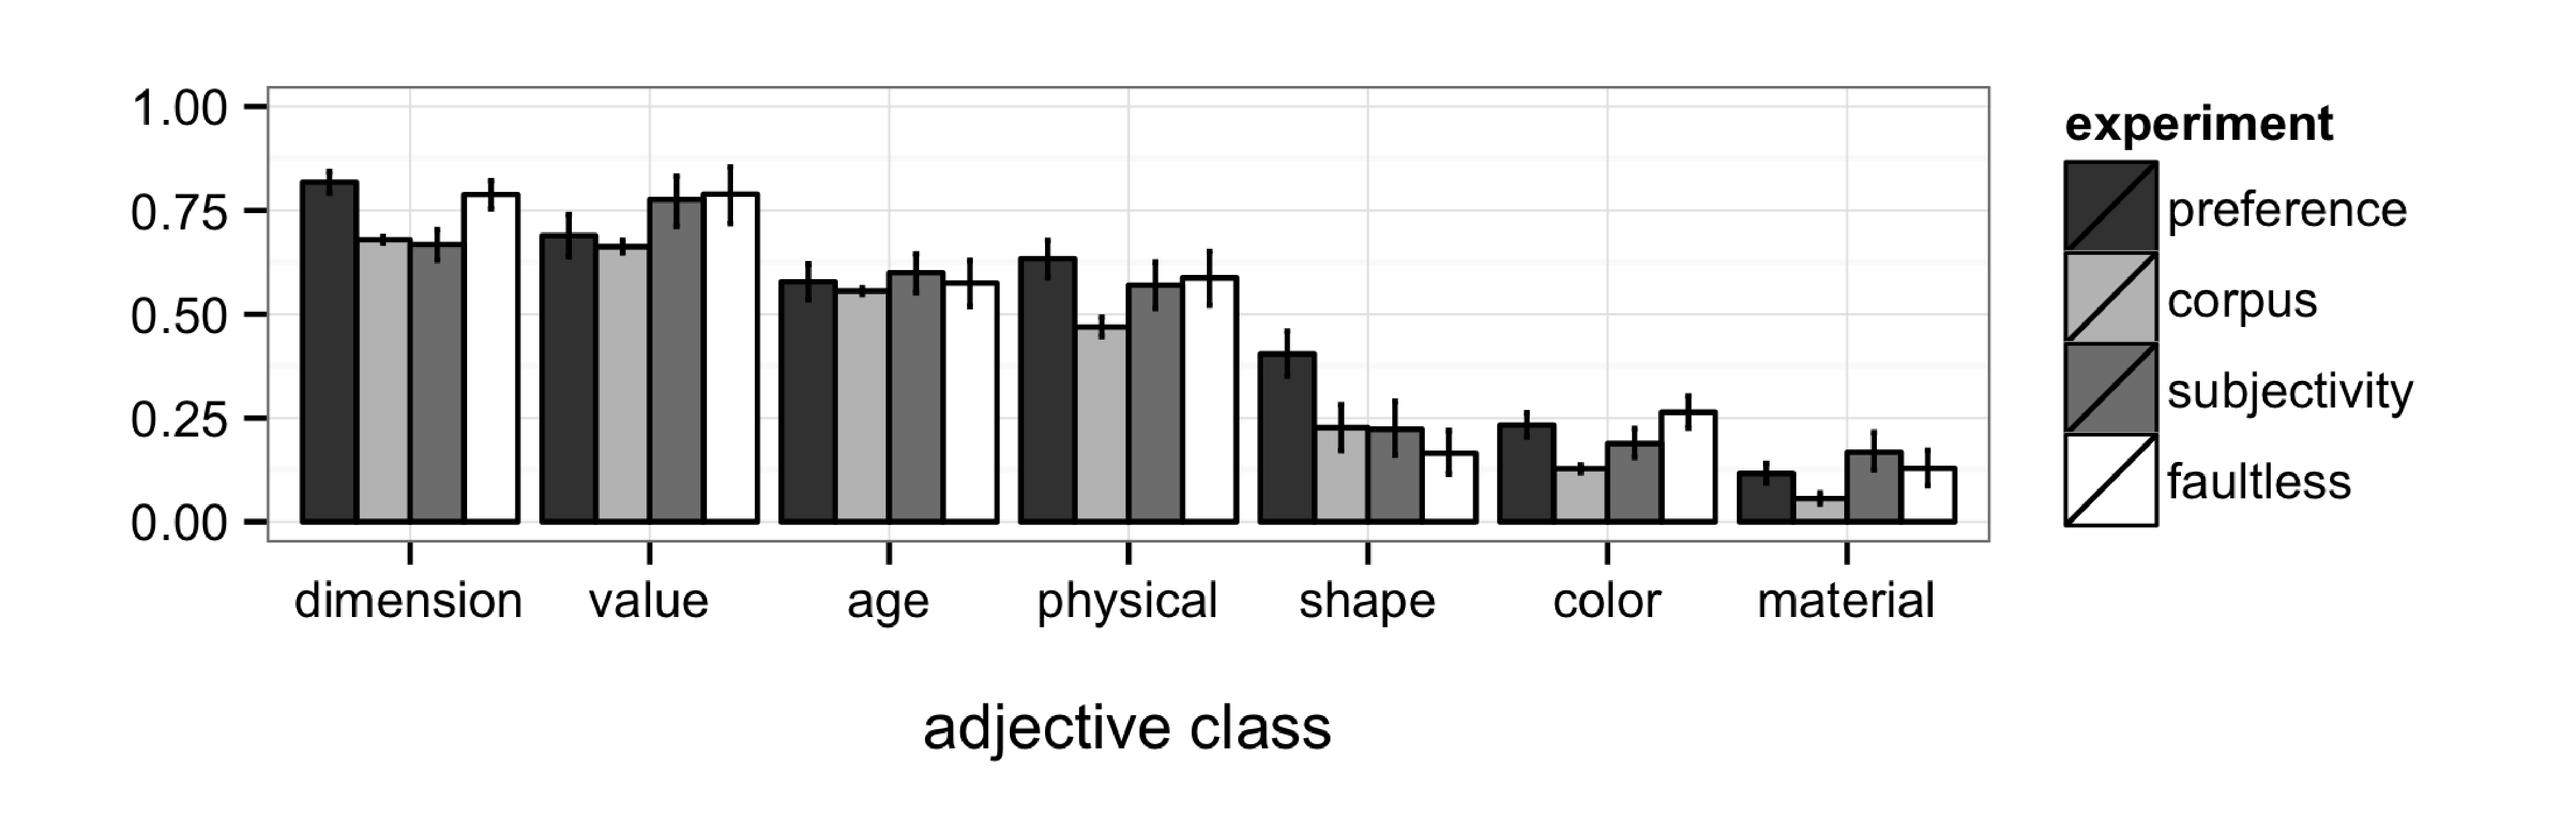
\includegraphics[width=.75\linewidth]{plots/expt_results-new.eps}}\par
	\caption{Mean distance from noun inferred from naturalness ratings (preference), mean distance from noun calculated from corpus counts (corpus),  mean faultless disagreement ratings (faultless), and mean subjectivity ratings (subjectivity) for adjectives grouped by their semantic class. Error bars represent bootstrapped 95\% confidence intervals drawn from 10,000 samples of the data \citep{DiCiccio1996}.}\label{results}
\end{figure*}

\begin{figure}
	\centering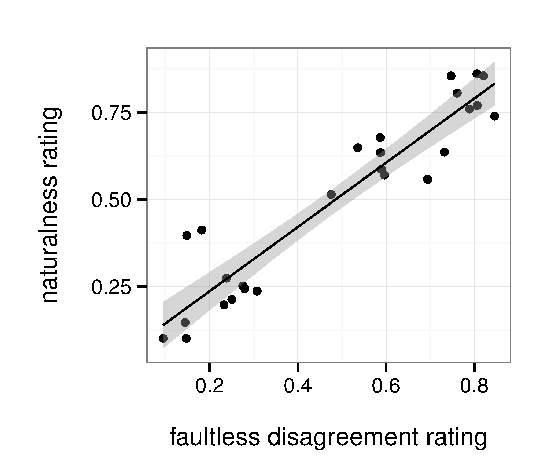
\includegraphics[width=2.8in]{plots/naturalness-faultless-new.eps}
	\caption{Mean naturalness ratings plotted against mean faultless disagreement scores for each of the 26 adjectives tested.}\label{naturalness-faultless-pred}
\end{figure}

\begin{figure}
	\centering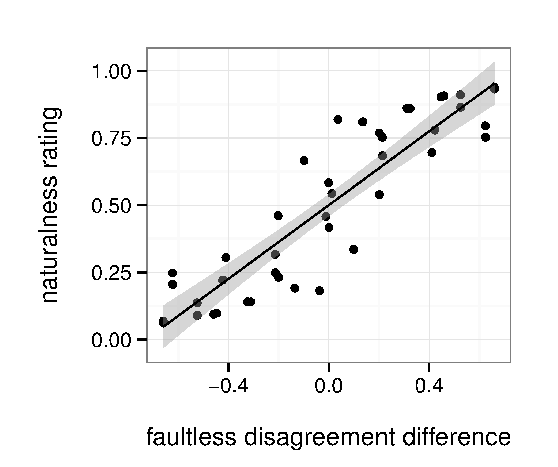
\includegraphics[width=2.8in]{plots/naturalness-faultless-configuration.eps}
	\caption{Mean configuration naturalness ratings plotted against faultless disagreement difference scores for each pair of adjective classes.}\label{naturalness-faultless}
\end{figure}


\begin{figure}[h]
	\centering
	\fbox{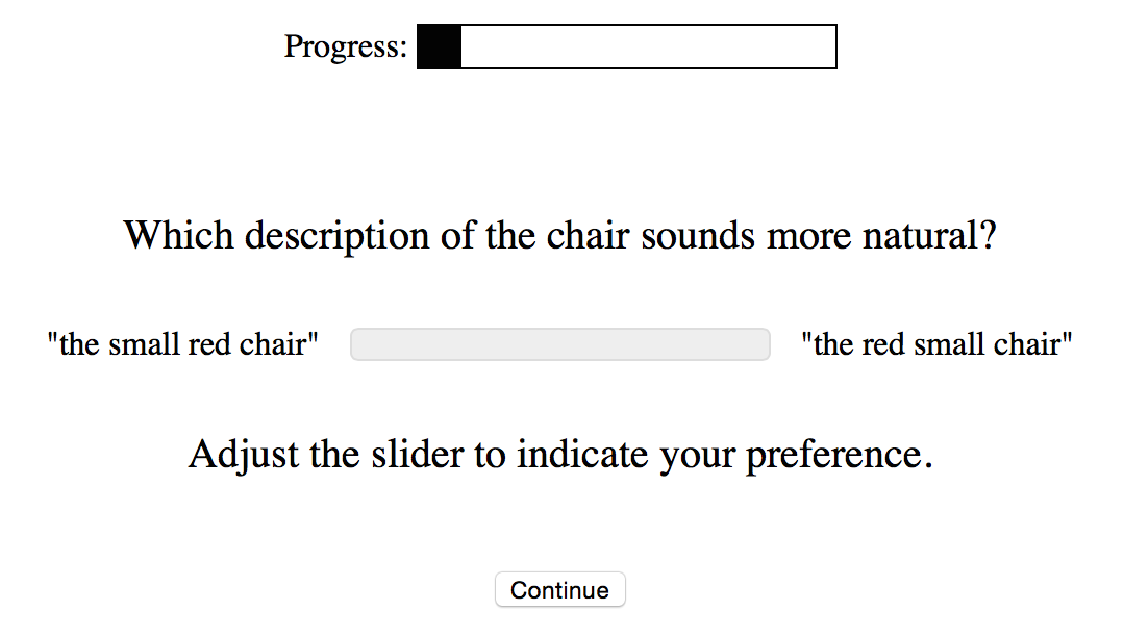
\includegraphics[width=3.3in]{images/order_trial.eps}}
	\caption{Example trial from Expt.\ 1; participants indicated the more natural of two adjective-adjective-noun descriptions on a sliding scale.}\label{order-trial}
\end{figure}

\begin{figure}[h]
	\centering
	\fbox{\includegraphics[width=3.75in]{images/faultless_trial.eps}}
	\caption{Example trial from Expt.\ 3; participants rated the potential for faultless disagreement between two speakers.}\label{faultless-trial}
\end{figure}

\begin{figure}[h]
	\centering
	\fbox{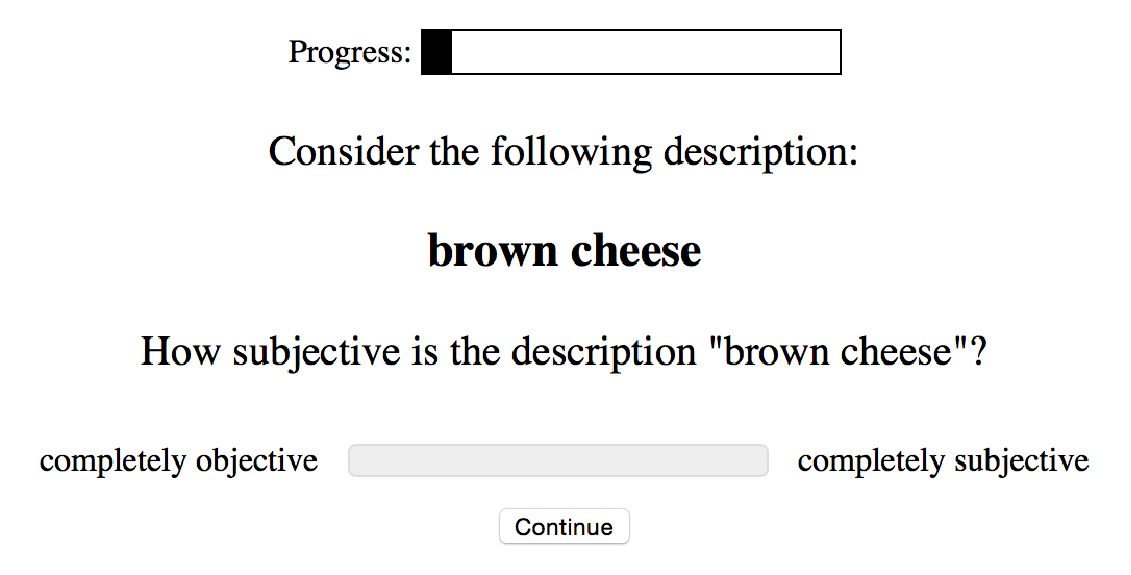
\includegraphics[width=3.3in]{images/subjectivity_trial.eps}}
	\caption{Example trial from Expt.\ 4; participants rated the subjectivity of adjective-noun object descriptions.}\label{subjectivity-trial}
\end{figure}

\begin{table}[t]
	\caption{Adjectives and their semantic classes tested in all experiments, and nouns and their classes tested in the behavioral experiments.}\label{stim-table}
	\centering{\footnotesize\begin{tabular}{@{\vrule height 10.5pt depth2pt  width0pt}llllll}
			{adjective}	&	{class}	&	{adjective}	&	{class}	&	{noun}	&	{class}	\\ \hline
			old	&	age	&	good	&	quality	&	apple	&	food	\\
			new	&	age	&	bad	&	quality	&	banana	&	food	\\
			rotten	&	age	&	round	&	shape	&	carrot	&	food	\\
			fresh	&	age	&	square	&	shape	&	cheese	&	food	\\
			red	&	color	&	big	&	size	&	tomato	&	food	\\
			yellow	&	color	&	small	&	size	&	chair	&	furniture	\\
			green	&	color	&	huge	&	size	&	couch	&	furniture	\\
			blue	&	color	&	tiny	&	size	&	fan	&	furniture	\\
			purple	&	color	&	short	&	size	&	TV	&	furniture	\\
			brown	&	color	&	long	&	size	&	desk	&	furniture	\\
			wooden	&	material	&	smooth	&	texture	\\				
			plastic	&	material	&	hard	&	texture	\\				
			metal	&	material	&	soft	&	texture	\\													
		\end{tabular}} 
	\end{table}







\section{Experiment 2}

Compositional (i.e., semantic) accounts of ordering preferences hold that the fundamental factor in predicting adjective ordering is whether or not an adjective is used to form a complex concept/subkind description: first you form the concept, then you modify it with additional adjectives \citep{McNally2004,svenonius2008}.\footnote{\cite{Bouchard2005} makes a similar claim, namely that the formation of complex concepts can override adjective ordering preferences.} 
This would imply that an interaction between the noun and a modifying adjective---whether they combine to form a complex concept---should have a large influence on adjective ordering. 
Indeed, a more general hypothesis is that \emph{some} interaction between a noun and adjective will influence how closely the adjective is placed to that noun. This interaction could be caused by concept-formation, differential subjectivity, or other factors. We tested for such an interaction in our original naturalness ratings and found that noun-specific naturalness did not explain any variance in ordering preference above and beyond adjective-level naturalness. However, there were two adjective-noun pairs in our data with trends in the predicted direction: the naturalness ratings for \emph{hard} and \emph{soft} suggested a preference to occur closer to the noun \emph{cheese}. (Plausibly because hard and soft cheeses are complex concepts.) While these adjective-noun interactions do not survive correction for multiple comparisons in our statistical analysis, they do indicate that a different set of materials might reveal by-noun effects on ordering preference. To follow up on this possibility, we re-ran our order preference and subjectivity experiments with a new set of materials that were chosen to maximize the probability of noun effects.


\subsection{Ordering preferences}

This experiment was a direct replication of our original naturalness ratings experiment (Experiment 1), using a different set of nouns. We chose nouns that we expected to form complex concepts with the given adjectives and therefore yield effects on ordering preferences.

\paragraph{Participants.}

We recruited 50 participants through Amazon.com's Mechanical Turk crowd-sourcing service. Participants were compensated for their participation.

\paragraph{Design and methods.}

The design was identical to our original naturalness ratings experiment: participants were asked to indicate which of two object descriptions sounded more natural, using a sliding scale. Each description featured a noun modified by two adjectives; description pairs contained the same words with the relative adjective order reversed (e.g., ``the big blue thing'' vs.~``the blue big thing''). Adjectives were chosen at random from the original set of 26. The nouns were a smaller set of five (compared to the original ten). Nouns were chosen to maximize the probability of detecting noun-specific effects on adjective ordering preferences. In particular, we expected that nouns that are likely to form complex concepts should be 
highly collocational with that adjective. We thus searched for nouns that occur in particular adjective-noun phrases more frequently than predicted by the individual noun and adjective probabilities; in other words, nouns whose adjective-noun combinations were under-predicted by their individual word probabilities. 

To find these nouns, we estimated the probability $p(A)$ of each adjective from our set of 26 by computing its relative frequency in an adjective-noun sequence in the BNC. We then computed the relative frequency of each noun $p(N)$ occurring in an adjective-noun sequence. Finally, we estimated the predicted joint probability of each adjective-noun combination by taking the product of each individual probability estimate: $\hat{p}(A,N) = p(A)\cdot p(N)$. Comparing  $\hat{p}(A,N)$ to the empirically estimated $p(A,N)$ establishes which adjective-noun combinations are under-predicted---more collocational---and thus likely to name complex concepts. We then restricted nouns to those 50 that maximize the observed range of under-predictedness while simultaneously requiring that each noun be attested to occur with at least 11 of the 26 adjectives; from these 50 nouns, we selected the following four: \emph{apple, cheese, eyes, hair}. (Recall that \emph{cheese} occurred in our original materials, where it suggested possible by-noun effects with the adjectives \emph{hard} and \emph{soft}.) To these four nouns we added a fifth: \emph{thing}.
While \emph{thing} did not occur in the top 50, it did occur naturalistically with the most adjectives (23) out of the set of 26, thus allowing it to serve as a filler for the various object descriptions. The selected nouns, together with the number of adjectives they occur with, their range of ratios of empirical to predicted joint probabilities, and their minimum / maximum ratios, are shown in Table \ref{tab:nouns}.

\renewcommand\thetable{S.\arabic{table}}
\begin{table}
\centering
\begin{tabular}{l c c c c}
\toprule
Noun & \# of adjectives & range of ratios & minimum ratio & maximum ratio\\
\midrule
thing & 23 & 10.4 & 0.1 & 10.5 \\
eyes & 18 & 120.6 & 0.12 & 120.7 \\
hair & 15 & 82.9 & 0.03 & 83.0 \\
cheese & 13 & 114.0 & 0.4 & 114.4 \\
apple & 11 & 674.0 & 1.1 & 675.1 \\
\bottomrule
\end{tabular}
\caption{For each chosen noun, the number of adjectives (out of 26) that it occurs with; and for each adjective $A$ that the noun occurs with, the range of ratios $p(A,N) / \hat{p}(A,N)$ (empirical to predicted probability of occurrence); the minimum ratio; and the maximum ratio.}
\label{tab:nouns}
\end{table}




\paragraph{Results.}

To evaluate the role of specific noun information in determining ordering preferences, we performed the same nested linear model comparison from our original naturalness ratings experiment. The models we compared predicted naturalness ratings either by \textsc{adjective} (i.e., the adjective farthest from the noun) only, or by \textsc{adjective} together with its interaction with \textsc{noun} (i.e., the modified noun).
The model comparison revealed that noun-specific ratings did not explain any additional variance in ordering preference beyond adjective-level ratings ($F(1,225) = 0.93, p < 0.75$).  Thus, we again fail to find evidence of noun-specific effects on ordering preferences, this time in our new materials. 

\subsection{Subjectivity}

We next set out to replicate the finding that subjectivity predicts adjective ordering preferences in our new materials.

\paragraph{Participants.}

We recruited 40 participants through Amazon.com's Mechanical Turk crowd-sourcing service. Participants were compensated for their participation.

\paragraph{Design and methods.}

This experiment was a direct replication of our original faultless disagreement subjectivity experiment (Experiment 3), using the new set of nouns from the previous experiment.

\paragraph{Results.}

To evaluate the power of subjectivity in predicting adjective ordering preferences, we compared our new adjective subjectivity scores to the naturalness ratings collected in the previous experiment. 
Faultless disagreement scores account for  84\% of the variance in the new naturalness ratings ($r^2$ 0.84, 95\% CI [0.64,  0.91]; Fig.~\ref{fig:faultless}). 
As with our original materials, more subjective adjectives are preferred farther from the noun; subjectivity again predicts adjective ordering preferences.


\renewcommand\thefigure{S.\arabic{figure}}
\begin{figure}
	\centering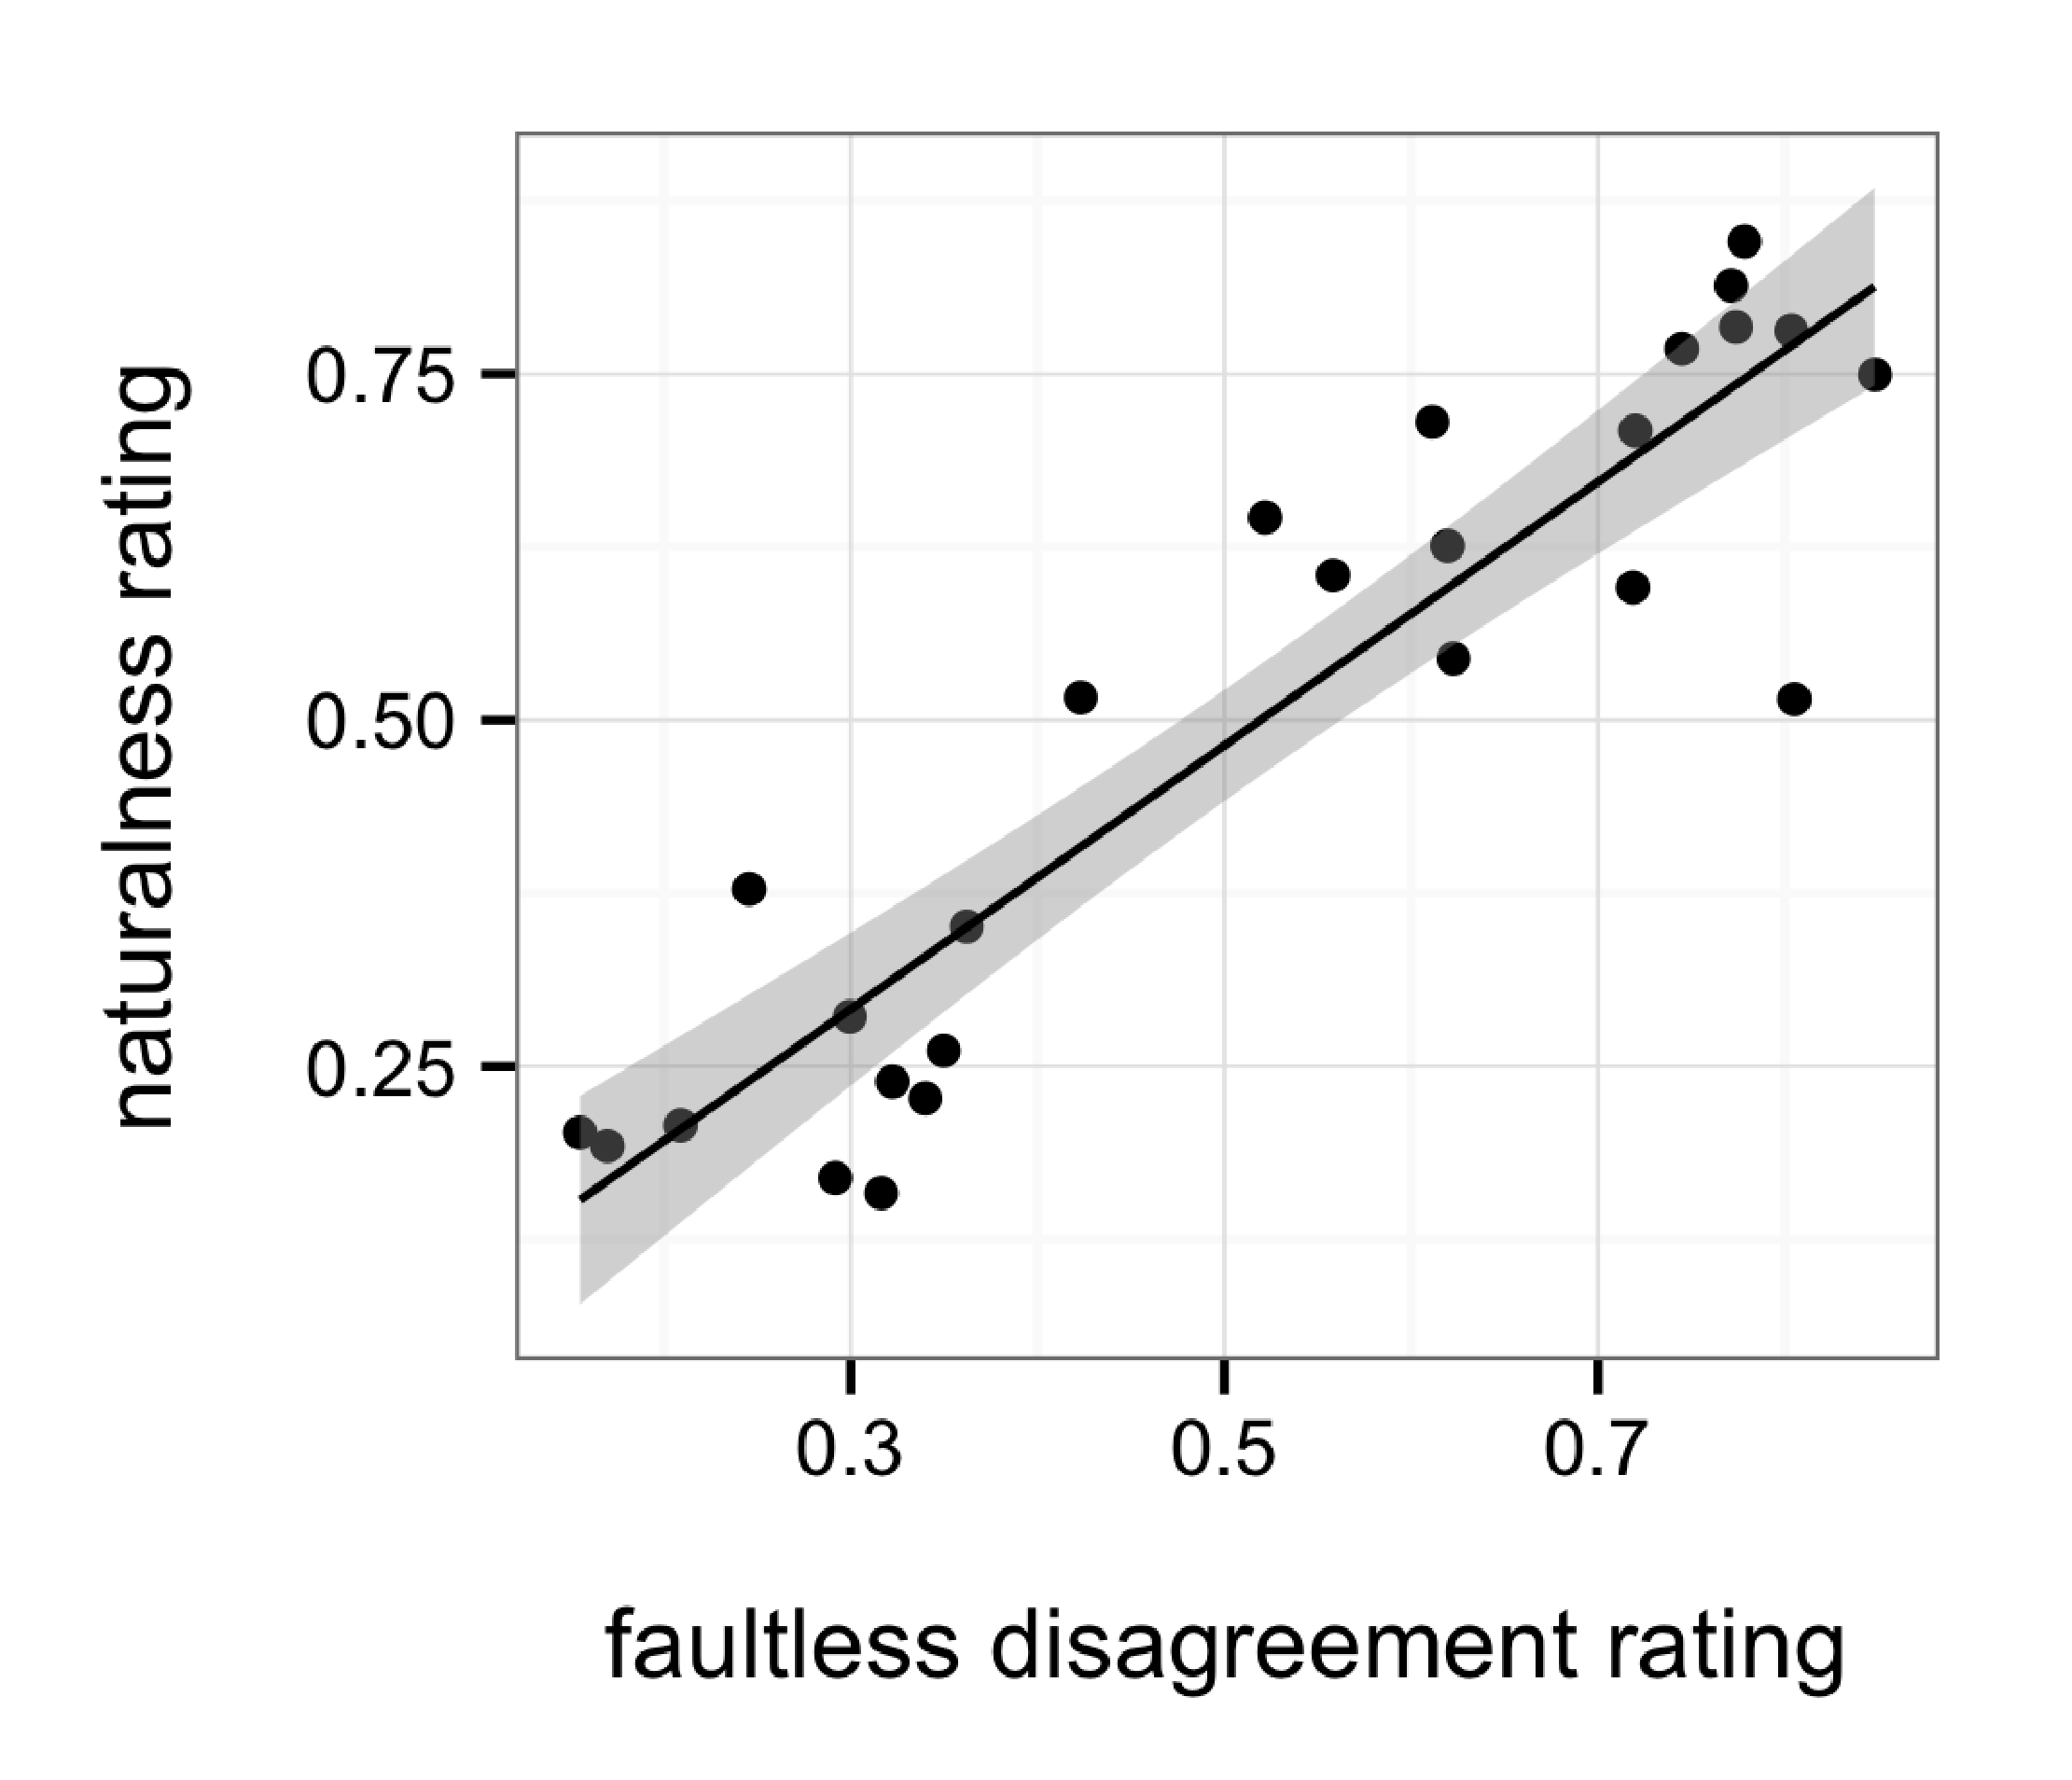
\includegraphics[width=2.8in]{plots/naturalness-faultless-new-nouns.eps}
	\caption{Mean naturalness ratings plotted against mean faultless disagreement scores for each of the 26 adjectives tested.}\label{fig:faultless}
\end{figure}

\subsection{Discussion}



\section{Experiment 3}




\section{General discussion}

Adjective ordering preferences have received considerable attention throughout the history of generative grammar and cognitive psychology, owing to their remarkable stability within and across languages. Something so robust, the reasoning goes, must evidence a deep principle of the cognitive architecture that shapes language. Yet while descriptions of the phenomenon abound, an explanation has proven elusive. Grammatical theories that posit a rigid syntax of adjective classes offer little more than a codification of the facts, and psychological approaches stumble when it comes to operationalizing the specific aspects of adjective meaning at play. 

In our investigation, we established two empirical constructs: the preferences themselves, which we measured using naturalness ratings and validated with corpus statistics; and adjective subjectivity, which we operationalized as potential for faultless disagreement and corroborated with a direct ``subjectivity'' measure. 
An adjective's semantics predict its distance from the modified noun, such that less subjective adjectives occur linearly closer to nouns they modify. 
This preference is not deterministic; non-preferred orderings of adjectives can serve a communicative purpose, for example to establish contrastiveness in discourse \citep{martin1969,Martin1970,hill1960,vendler1963}. This constrastiveness follows straightforwardly from a manner implicature \cite{levinson2000}: marked forms (i.e., non-preferred orderings of adjectives) yield marked interpretations (i.e., atypical modification constituency). The work lies in determining the preferred orderings from which  contrastive uses depart. Indeed, many other situational factors are likely to influence ordering (e.g., phonological shape, noun semantics, word and bi-gram frequencies \cite{wulff2003}); it is the more general tendencies we are concerned with here.

Adjectives are just one of many elements that may occur in complex nominal constructions. Other classes of elements include demonstratives (e.g., \emph{this} and \emph{that}) and numerals. In his Universal 20, Greenberg observes that the relative order of these higher-order classes is also stable cross-linguistically \citep{greenberg1963,Culbertson2014}, suggesting that subjectivity interacts with additional constraints from semantic composition in the determination of word order. Beyond nominals, adverbs (e.g., \emph{honestly}, \emph{probably}, \emph{carefully}) are reported to exhibit regular orderings cross-linguistically \cite{cinque1999,ernst2002}. Understanding these orderings would likely benefit from a systematic empirical treatment similar to the one we have advanced here.


Our results suggest that ordering preferences likely emerge, at least partially, from a desire to place less subjective content closer to the substantive head of a nominal construction (i.e., closer to the modified noun). 
For now we can only speculate about the ultimate source of this desire: Subjective content allows for miscommunication to arise if speakers and listeners arrive at different judgments about a property description. Hence, less subjective content is more useful at communicating about the world. 
An explanation along these lines, based on pressures to facilitate successful reference resolution, would have to depend on the hierarchical, not linear, ordering of adjectives (cf.~the mirroring of preferences in pre- and post-nominal languages). 
Whatever its source, the success of subjectivity in predicting adjective ordering preferences provides a compelling case where linguistic universals, the regularities we observe in adjective ordering, emerge from cognitive universals, the subjectivity of the properties that the adjectives name.


  \bibliographystyle{chicago} 
  \bibliography{adjectives.bib}


\end{document}














